\chapter{Suggested Algorithms}
\label{chapter_solutions}

% **************************** Define Graphics Path **************************
\ifpdf
    \graphicspath{{Chapter4/Figs/Raster/}{Chapter4/Figs/PDF/}{Chapter4/Figs/}}
\else
    \graphicspath{{Chapter4/Figs/Vector/}{Chapter4/Figs/}}
\fi

This chapter presents the suggested learning algorithms for predictive models in detail. Section \ref{sec_predictiveEpisodeMining} explains predictive episode mining, an approach that aims to discover predictive episodes in the stream. Section \ref{sec_FeatureBasedStreamWindowClassification} explains the idea of feature based stream window classification in order to predict event occurrences. 

\section{PERMS - Predictive Episode Rule Mining in Streams}
\label{sec_predictiveEpisodeMining}
The first suggested algorithm is called the PERMS algorithm, short for \textbf{P}redictive \textbf{E}pisode \textbf{R}ule \textbf{M}ining in \textbf{S}treams.

\subsection{Basic Ideas and Definitions}
In order to fully explain the algorithm we first need to define what we mean by predictive episode rules.

\begin{mydef}
\label{def_predictiveEpisode}
\textbf{Predictive Episode Rule} An episode $\alpha$ is called a predictive episode rule for event $A \in \Sigma$ if $\alpha$ has the form $\beta \rightarrow A$ where $\beta$ is an episode. 
\end{mydef}

TODO: limit length/duration 

In the context of a predictive episode rule $\alpha = \beta \rightarrow A$ we also refer to $\beta$ as the prefix and to $A$ as the suffix of $\alpha$. 
The basic idea of the prediction algorithm using predictive episode rules is rather simple. If given a set $P$ of predictive episode rules, we monitor the stream and whenever we detect the prefix of an episode in $P$ we predict an occurrence of $A$. The idea is similar to the mining of sequential rules or rule-based classification (TODO: cite).
Of course there is an infinite amount of predictive episode rules for an event type, finding those predictive episode rules that are actually useful for predicting the occurrence of an event is the main task when building (training) the model. The use case here is very similar to the related work that deals with the constraint based mining of episode rules (TODO: cite), where episode rules are mined in order to discover dependencies between earthquakes. There are two main important differences that make the approach used by the authors (TODO: name them) impractical.

\begin{itemize}
 \item We are interested in episode rules of one specific type (those predicting the desired event $A$), thus it is not necessary to mine all frequent episode rules in the stream.
 \item We are dealing with data in a streaming environment, meaning we can neither analyze the whole data, nor make multiple passes over the entire stream.
\end{itemize}

In order to describe how the set $P$ is built we first need to define support and confidence for predictive episode rules.

\begin{mydef}
\label{def_support}
\textbf{Support} The support of a predictive episode $\alpha = \beta \rightarrow A$ is defined as $freq(\alpha)$, where $freq$ is a frequency measure for episodes, as discussed in sections \ref{subsec_windowBased} and \ref{subsec_otherFrequency}. TODO: not really frequency but support
\end{mydef}

\begin{mydef}
\label{def_confidence}
\textbf{Confidence} The confidence of a predictive episode $\alpha = \beta \rightarrow A$ is defined as $\frac{freq(\alpha)}{freq(\beta)}$, where $freq$ is a frequency measure for episodes.
\end{mydef}

The intention is clear and similar to the mining of classic association rules (TODO: cite): If a rule has a high confidence, it means that the prefix of the rule rarely occurs without its suffix $A$, meaning there is a high chance that this is a true predictor for the event $A$. Thus the goal of PERMS is to find a set of predictive episode rules $P$ that have a very high confidence and are above a certain support limit.

\subsection{Choice of training data and frequency measure}
Recall that in streaming applications it is impossible for to analyze the whole stream as one sequence using multiple passes. Thus, when presented with a stream any prediction or forecasting algorithm first needs to take some time to study the stream and extract training data to build the model. So if given an annotated event stream, how do we determine the training data? As it was described in section \ref{sec_episodeMiningBackground} the data basis for episode mining is one very long sequence. Thus the first simple approach would be to simply record the stream as a sequence until we have reached a number of desired elements or run out of memory. The recorded sequence would then be the training sequence from which the predictive episode rules can be mined. This approach is visualized in figure \ref{trainingDataNaive}.

\begin{figure}[h]
	\centering
  	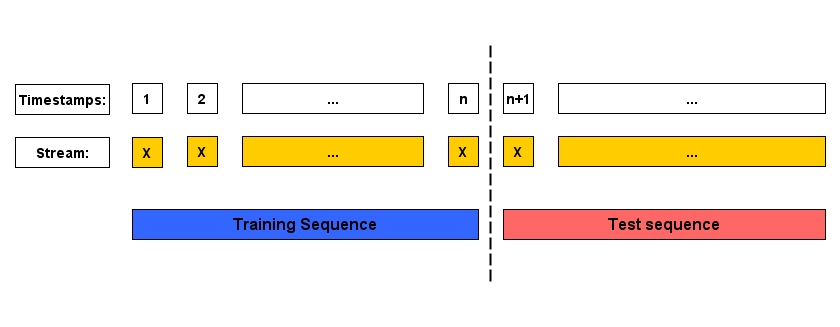
\includegraphics[width=\textwidth]{trainingDataNaive}
	\caption{Visualization of a simple split of the stream into a training segment at the beginning, followed by a (potentially endless) test phase}
	\label{fig_trainingDataNaive}
\end{figure}

The disadvantage of this naive approach is that there is no guarantee about the number of occurrences of the event we aim to predict. Say we want to predict $A$ and $A$ is rather sparse in the beginning of the stream, then we will have a very small data basis to extract predictive episode rules for $A$ and thus will likely not succeed. 
A better approach is to scan the stream for occurrences of the event $A$ and whenever an event of type $A$ enters the window we store the current window in a list until we have a sufficient number of windows. This approach is visualized in figure TODO. This approach guarantees that we have a sufficient data basis to mine predictive episodes, however it does limit us to frequency measures that are based on windows. 

\begin{figure}[h]
	\centering
  	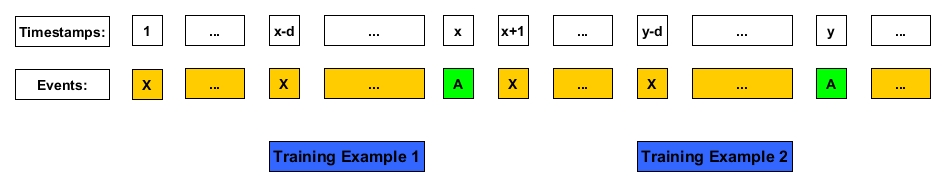
\includegraphics[width=\textwidth]{trainingDataWindowsOfA}
	\caption{Visualization of using fixed windows that precede the target event as training examples. Predictive episodes can be mined from the windows that are extracted from the stream as shown above.}
	\label{fig_trainingDataNaive}
\end{figure}

The obvious and very big disadvantage is that there are no negative examples in the training sample taken from the stream. Each window ends with the target event $A$, thus every episode mined from the windows can have $A$ appended as a suffix and thus every predictive episode rule will have a confidence of $1.0$. This means that selection via confidence is meaningless, since we have seen no negative examples, meaning windows that are not followed by $A$. However negative examples can be extracted from the stream in a similar manner. This is the basic idea behind the training data selection in PERMS. It is visualized in figure \ref{fig_trainingDataPositiveAndNegativeWindows}. 

\begin{figure}[h]
	\centering
  	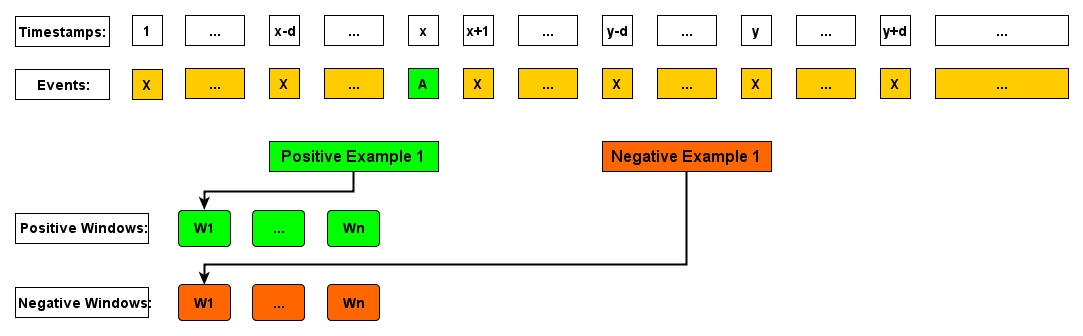
\includegraphics[width=\textwidth]{trainingDataPositiveAndNegativeWindows}
	\caption{Extracting positive and negative example windows from the stream.}
	\label{fig_trainingDataNaive}
\end{figure}

There are still some issues with this approach that can be detrimental to the predictive performance of the model. One issue is that, in the simple standard scenario extract an equal amount of positive and negative windows from the stream with no respect to the original distribution. If $A$ occurs very rarely, having an equal amount of positive and negative examples in the training data does not reflect the original event distribution in the stream. If that is the case, this can be fixed by including a number of negative examples that is proportionate to the original distribution (which is either known or learned while extracting the training data). However it is unclear if that would actually have a significantly positive effect on the performance of the resulting model.



TODO: define negative and positive windows!




\subsection{PERMS Parameters and Pseudocode}

The PERMS algorithm uses the following user-defined parameters:

\begin{itemize}
	\item \textbf{$d$} - the (temporal) size of the sliding window. This also implies that all windows which the predictive episode rules will be mined from will exactly have duration $d$. TODO: talk about episode duration?	
	\item \textbf{$m$} - the number of windows to mine the predictive episode rules from. Basically the sample size we take from the stream.
	\item \textbf{$s$} - the minimum support that predictive episode rules must have to be considered for the model (rules with support $s$ or higher are frequent).
	\item \textbf{$|P|$} - the desired size of the final set of predictive episodes.
\end{itemize}


The basic idea of the PERMS algorithm is the following:
We start at the beginning of the stream and keep a sliding window of a user defined size $d$ in memory. Whenever an event of type $A$ enters the window we store the current window in a list until we have a sufficient number of windows ($m$). Additionally we also store $m$ windows that do not contain $A$ and were also not followed by $A$ in the near future. Once we have enough windows, we can start to mine serial and parallel episodes from the windows preceding $A$ that have support $s$ or higher. Afterwards we rank the discovered rules by confidence, keep the $|P|$ episodes with the highest confidence and return them as the set of predictive episodes $P$.
The subsequent application of the predictive model to the stream is very simple: If an episode $\alpha \in P$ occurs in the current sliding window output $1$ and otherwise output $0$ for the current sliding window.
TODO: pseudocode plus images

\section{Feature Based Stream Window Classification}
\label{sec_FeatureBasedStreamWindowClassification}



\section{Evolving the models with the stream}